%%%%%%%%%%%%%%%%%%%%%%%%%%%%%%%%%%%%%%%%%%%%%%%%%%%%%%%%%%%%%%%%
%                                                              %
%                                                              %
% Macallyster S. Edmondson                                     %
%                                                              %
% ECE351-53                                                    %
%                                                              %
% Lab #7                                                       %
%                                                              %
% 03/08/2022                                                   %
%                                                              %
% Straightforward layout, broken into sections, uses many      %
% common libraries. Note, Hyperlinks are not highlighted.      %
%                                                              %
%%%%%%%%%%%%%%%%%%%%%%%%%%%%%%%%%%%%%%%%%%%%%%%%%%%%%%%%%%%%%%%%

%%%%%%%%%%%%%%%%%%%%%%%%%%%%%%%%%%%%%%%%%%%
%%% DOCUMENT PREAMBLE %%%
\documentclass[12pt]{report}
\usepackage[english]{babel}
%\usepackage{natbib}
\usepackage{url}
\usepackage[utf8x]{inputenc}
\usepackage{amsmath}
\usepackage{graphicx}
\graphicspath{{./images/}}
\usepackage{parskip}
\usepackage{fancyhdr}
\usepackage{vmargin}
\usepackage{listings}
\usepackage[hidelinks]{hyperref}
\usepackage{xcolor}
\usepackage[nodayofweek]{datetime}
\usepackage[section]{placeins}
\usepackage{pdfpages}
\definecolor{codegreen}{rgb}{0,0.6,0}
\definecolor{codegray}{rgb}{0.5,0.5,0.5}
\definecolor{codeblue}{rgb}{0,0,0.95}
\definecolor{backcolour}{rgb}{0.95,0.95,0.92}
\lstdefinestyle{mystyle}{
backgroundcolor=\color{backcolour},
commentstyle=\color{codegreen},
keywordstyle=\color{codeblue},
numberstyle=\tiny\color{codegray},
stringstyle=\color{codegreen},
basicstyle=\ttfamily\footnotesize,
breakatwhitespace=false,
breaklines=true,
captionpos=b,
keepspaces=true,
numbers=left,
numbersep=5pt,
showspaces=false,
showstringspaces=false,
showtabs=false,
tabsize=2
}
\lstset{style=mystyle}
\setmarginsrb{3 cm}{2.5 cm}{3 cm}{2.5 cm}{1 cm}{1 cm}{1 cm}{1.5 cm}
\title{Lab \#7 Report}
% Title
\author{Macallyster S. Edmondson}
% Author
\newdate{date}{08}{03}{2022}
\date{\longdate\displaydate{date}}
% Date
\makeatletter
\let\thetitle\@title
\let\theauthor\@author
\let\thedate\@date
\makeatother
\pagestyle{fancy}
\fancyhf{}
\rhead{\theauthor}
\lhead{\thetitle}
\lfoot{Page: \thepage}
\rfoot{\thedate}
\fancypagestyle{customplain}{ %Used for default pages with plain style to keep overall document consistency
  \fancyhf{}
  \renewcommand{\headrulewidth}{0pt} %Remove bar from top of page
  \lfoot{Page: \thepage}
}
\fancypagestyle{titlepage}{ %Used for default pages with plain style to keep overall document consistency
  \fancyhf{}
  \renewcommand{\headrulewidth}{0pt} %Remove bar from top of page
  \cfoot{\thedate}
}
\fancypagestyle{customblank}{ %Used for default pages with plain style to keep overall document consistency
  \fancyhf{}
  \renewcommand{\headrulewidth}{0pt} %Remove bar from top of page
}
%%%%%%%%%%%%%%%%%%%%%%%%%%%%%%%%%%%%%%%%%%%%
\begin{document}
%%%%%%%%%%%%%%%%%%%%%%%%%%%%%%%%%%%%%%%%%%%%%%%%%%%%%%%%%%%%%%%%%%%%%%%%%%
%%%%%%%%%%%%%%%
\begin{titlepage}\thispagestyle{titlepage}
\centering
%\vspace*{0.5 cm}

\includegraphics[scale = 0.12]{univ-logo.png}\\[1.0 cm]
%University of Idaho
\begin{center}    \textsc{\Large   ECE 351 - Section \#53 }\\[2.0 cm]
\end{center}% University Name

%Lab Report
\rule{\linewidth}{0.2 mm} \\[0.4 cm]
{ \huge \bfseries \thetitle}\\
\rule{\linewidth}{0.2 mm} \\[0.5 cm]
\textsc{\Large Block Diagrams and System Stability }\\[1.5 cm] % Course 
\begin{minipage}{0.4\textwidth}
\begin{flushleft} \large
\emph{Submitted To:}\\
Kate Antonov\\ \small
University of Idaho\\
kantonov@uidaho.edu\\
\hfill
\end{flushleft}
\end{minipage}~
\begin{minipage}{0.4\textwidth}
\begin{flushright} \large
\emph{Submitted By :} \\
\theauthor \\ \small
University of Idaho\\
edmo7033@vandals.uidaho.edu\\
\href{http://github.com/mac-edmondson}{github.com/mac-edmondson}\\
\end{flushright}
\end{minipage}\\[2 cm]
\vfill
\end{titlepage}
%%%%%%%%%%%%%%%%%%%%%%%%%%%%%%%%%%%%%%%%%%%%%%%%%%%%%%%%%%%%%%%%%%%%%%%%%%
%%%%%%%%%%%%%%%
\tableofcontents\thispagestyle{customplain}
\pagebreak
%%%%%%%%%%%%%%%%%%%%%%%%%%%%%%%%%%%%%%%%%%%%%%%%%%%%%%%%%%%%%%%%%%%%%%%%%%
%%%%%%%%%%%%%%%
\renewcommand{\thesection}{\arabic{section}}
\section{Introduction}
The goal of this weeks lab was to become familiar with Laplace-domain block diagrams and use the factored form of the transfer function to determine system stability.
These concepts have been covered in class and applying them using computational tools was a great exercise.
Yet again, this lab was completed using \textit{Python} through the \textit{Spyder-IDE}. The packages used in the completion of this lab were \texttt{numpy} for 
definitions of mathematical functions, \texttt{matplotlib.pyplot} to plot outputs of functions, and \texttt{scipy.signal} to perform convolutions for reasons discussed
throughout the report.

All code for this lab, including this report, can be found on \href{http://github.com/mac-edmondson}{my Github}.
\section{Equations}\label{section: eq}
The equations used within this lab are shown in this section. The equations will be referenced by number throughout the rest of the report.
\begin{equation}\label{eq: ol_tran}
  \begin{aligned}[c]
    H_{OL}(s) = \frac{(s+9)(s+4)}{(s+2)(s+4)(s-8)(s+3)(s+1)}
  \end{aligned}
\end{equation}
\begin{equation}\label{eq: cl_tran}
  \begin{aligned}[c]
    H_{CL}(s) = \frac{A_{num}G_{num}}{A_{den}G_{den} + A_{den}B_{num}G_{num}}
  \end{aligned}
\end{equation}

\section{Methodology}
\subsection{Lab: Part 1}\label{Section: Part1}
In part 1 of this lab, we calculated the Open-Loop transfer function of the block-diagram system given in the lab handout by hand and using Python.
The calculated equation can be seen in Equation \ref{eq: ol_tran}. This was verified with Python using the \texttt{scipy.signal.tf2zpk()} function
and the \texttt{scipy.signal.convolve()} function, giving the poles, zeros and expanded numerator and denominator coefficients of the total transfer function
(Results seen in: Figure \ref{fig: p1t2}). As can be seen, the OL transfer function is unstable due to at least one pole being in the RHP. This can be obviously seen
in the graph for this transfer function (Figure \ref{fig: p1t5}) since \(h(t)\to\infty\) as \(t\to 8\). 

Below can be seen the code implementation of the tasks carried out in Part 1 of this lab.

\begin{lstlisting}[language=Python, basicstyle=\footnotesize]
  # PART 1
print("### PART 1 ###\n")

# 1/2
zG, pG, kG = spsig.tf2zpk([1, 9], [1, -2, -40, -64])
zA, pA, kA = spsig.tf2zpk([1, 4], [1, 4, 3])
# zB, pB, kB = np.roots(1, 26, 168)

print("G(s): z = ", zG, "p = ", pG)
print("A(s): z = ", zA, "p = ", pA)

#3/4 (Open Loop HT = A*G)
num = spsig.convolve([1, 9], [1, 4])
den = spsig.convolve([1, -2, -40, -64], [1, 4, 3])
print("\nOpen Loop Numerator: ", num)
print("Open Loop Denominator: ", den)

#5
tout, y1 = spsig.step(spsig.lti(num, den))
plt.figure(figsize = (10, 11))
plt.subplot(1, 1, 1)
plt.plot(tout, y1, "b-")
plt.grid()
plt.ylabel('h(t) (Open Loop)')
plt.xlabel('t')
plt.title('Open Loop TF Step Response')
\end{lstlisting}

\subsection{Lab: Part 2}\label{section: Part2}
In Part 2 of this lab, we again used the \texttt{scipy.signal.tf2zpk()} and \\\texttt{scipy.signal.convolve()} functions. This time, they were used to find the
closed-loop transfer function of the block-diagram system given in the lab handout. Rather than doing a hand calculation to find the exact transfer function,
the transfer function was found symbolically, seen in equation \eqref{eq: cl_tran}. This symbolic equation made finding the transfer function of the closed-loop
system very easy and the expanded numerator and denominator coefficient matrices can be seen in Figure \ref{fig: p1t2}, while the graph of the transfer function
can be seen in Figure \ref{fig: p2t4}. Both outputs tell us that the closed-loop transfer function is stable!

Below can be seen the code implementation of the tasks carried out in Part 2 of this lab.
\begin{lstlisting}[language=Python, basicstyle=\footnotesize]
  #PART 2
  print("\n### PART 2 ###\n")
  #1/2
  
  numG = [1, 9]
  denG = [1, -2, -40, -64]
  
  numA = [1, 4]
  denA = [1, 4, 3]
  
  B = [1, 26, 168]
  
  numMain = spsig.convolve(numA, numG)
  denT1 = spsig.convolve(denG, denA)
  denT2 = spsig.convolve(denA, spsig.convolve(B, numG))
  denMain = denT1 + denT2
  
  #3
  print("Closed Loop Numerator: ", numMain)
  print("Closed Loop Denominator: ", denMain)
  z,p,k = spsig.tf2zpk(numMain, denMain)
  print("G(s): z = ", z)
  
  #4
  tout, y1 = spsig.step(spsig.lti(numMain, denMain))
  plt.figure(figsize = (10, 11))
  plt.subplot(1, 1, 1)
  plt.plot(tout, y1, "b-")
  plt.grid()
  plt.ylabel('h(t) (Closed Loop)')
  plt.xlabel('t')
  plt.title('Closed Loop TF Step Response')
\end{lstlisting}

\section{Results}\label{section: Results}
The results of this lab are very straightforward. The implementation of all functions worked as expected and the results are as expected.

The deliverables for Parts 1 \& 2 of this lab can be seen in Figures \ref{fig: p1t2}, \ref{fig: p1t5}, \& \ref{fig: p2t4}, below.
\\
\begin{figure}[h!]
  \centering
  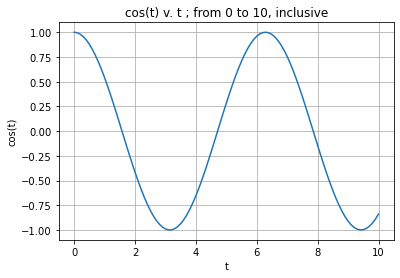
\includegraphics[scale=.7]{p1t2.png}
  \caption{Program Output}
  \label{fig: p1t2}
\end{figure}
\begin{figure}[h!]
  \centering
  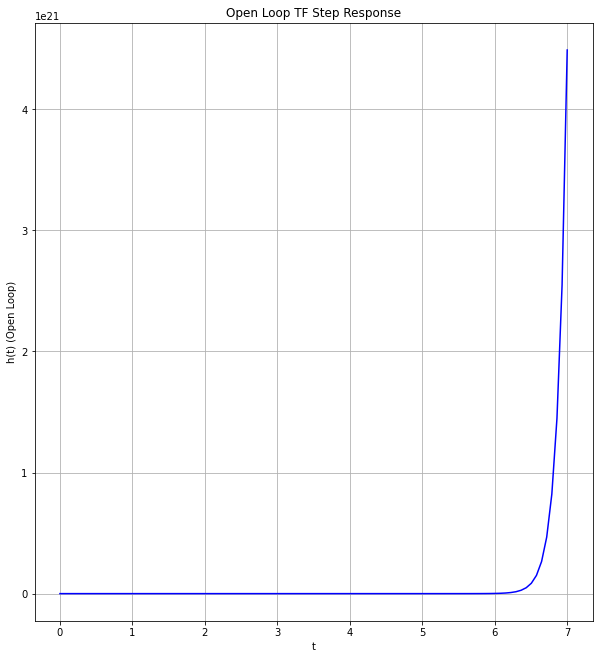
\includegraphics[scale=0.5]{p1t5.png}
  \caption{Part 1, Task 5}
  \label{fig: p1t5}
\end{figure}
\begin{figure}[h!]
  \centering
  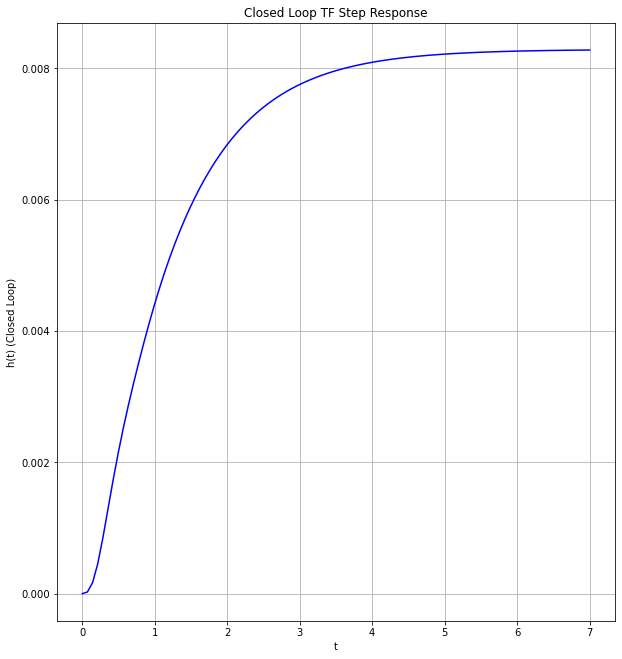
\includegraphics[scale=0.5]{p2t4.png}
  \caption{Part 2, Task 4}
  \label{fig: p2t4}
\end{figure}
\section{Error Analysis}\label{section: ErAn}
No sources of error were seen throughout this lab, and I did not run into any real problems while implementing anything lab lab asked. Part 2 was time consuming
and without a lab TA to tell me that my graph was correct, I'm not sure how I would know I did it right. I wish this was something included in this lab.
\section{Questions}
\begin{enumerate}
  \item Using the \texttt{scipy.signal.convolve()} function to find the expanded form of the numerator or denominator works due to the fact that all coefficient 
  matrices represent coefficients for s-domain functions. As we know, convolution in the time-domain is the same as multiplication in the s-domain. With that in 
  mind, the convolution function we made in \textbf{Lab 3} would not have worked as it was made strictly based on the summation definition and only worked to graph
  convolutions discretely, not perform "symbolic" math as with the \texttt{scipy} function.
  \item As seen throughout this lab, the open-loop transfer function is unstable and the closed-loop transfer function was stable. This may be the reason you choose
  to have feedback in a system. For any system to be implemented realistically, it should be stable. Feedback could be used to make an open-loop system stable.
  \item The \texttt{scipy.signal.tf2zpk()} function is used to find the zero, pole, and gain of transfer function. The \texttt{scipy.signal.residue()} function takes
  the numerator and denominator coefficients of a function and performs partial fraction expansion, returning
  the residue (denominator term) and poles for each term in the PFE. (See \href{https://docs.scipy.org/doc/scipy/reference/}{scipy reference}.)
  \item It is possible for any system to be stable or unstable. It just depends on the transfer functions that go into making the overall transfer function. 
 \(\frac{Y(s)}{F(s)}\) . This goes along with my answer to Question 3.
  \item See the end of \nameref{section: ErAn} for some feedback on the lab. Other than that, purpose, deliverables, and expectations were very clear for this lab.
\end{enumerate}
\section{Conclusion}
In conclusion, I feel this lab was very successful. The implementation of the code in this lab was quite simple and I really enjoyed seeing how you could
find the total transfer function with some symbolic math and Python. All in all, I am very satisfied with what this lab has taught me and feel it was an 
excellent use of time.
\newpage
\thispagestyle{customblank}
\section{Attachments}\label{section: Attachments}
No attachments for this lab.
% \centering\begin{enumerate}
%   \item Pre-Lab
% \end{enumerate}
\vspace*{\fill}

% 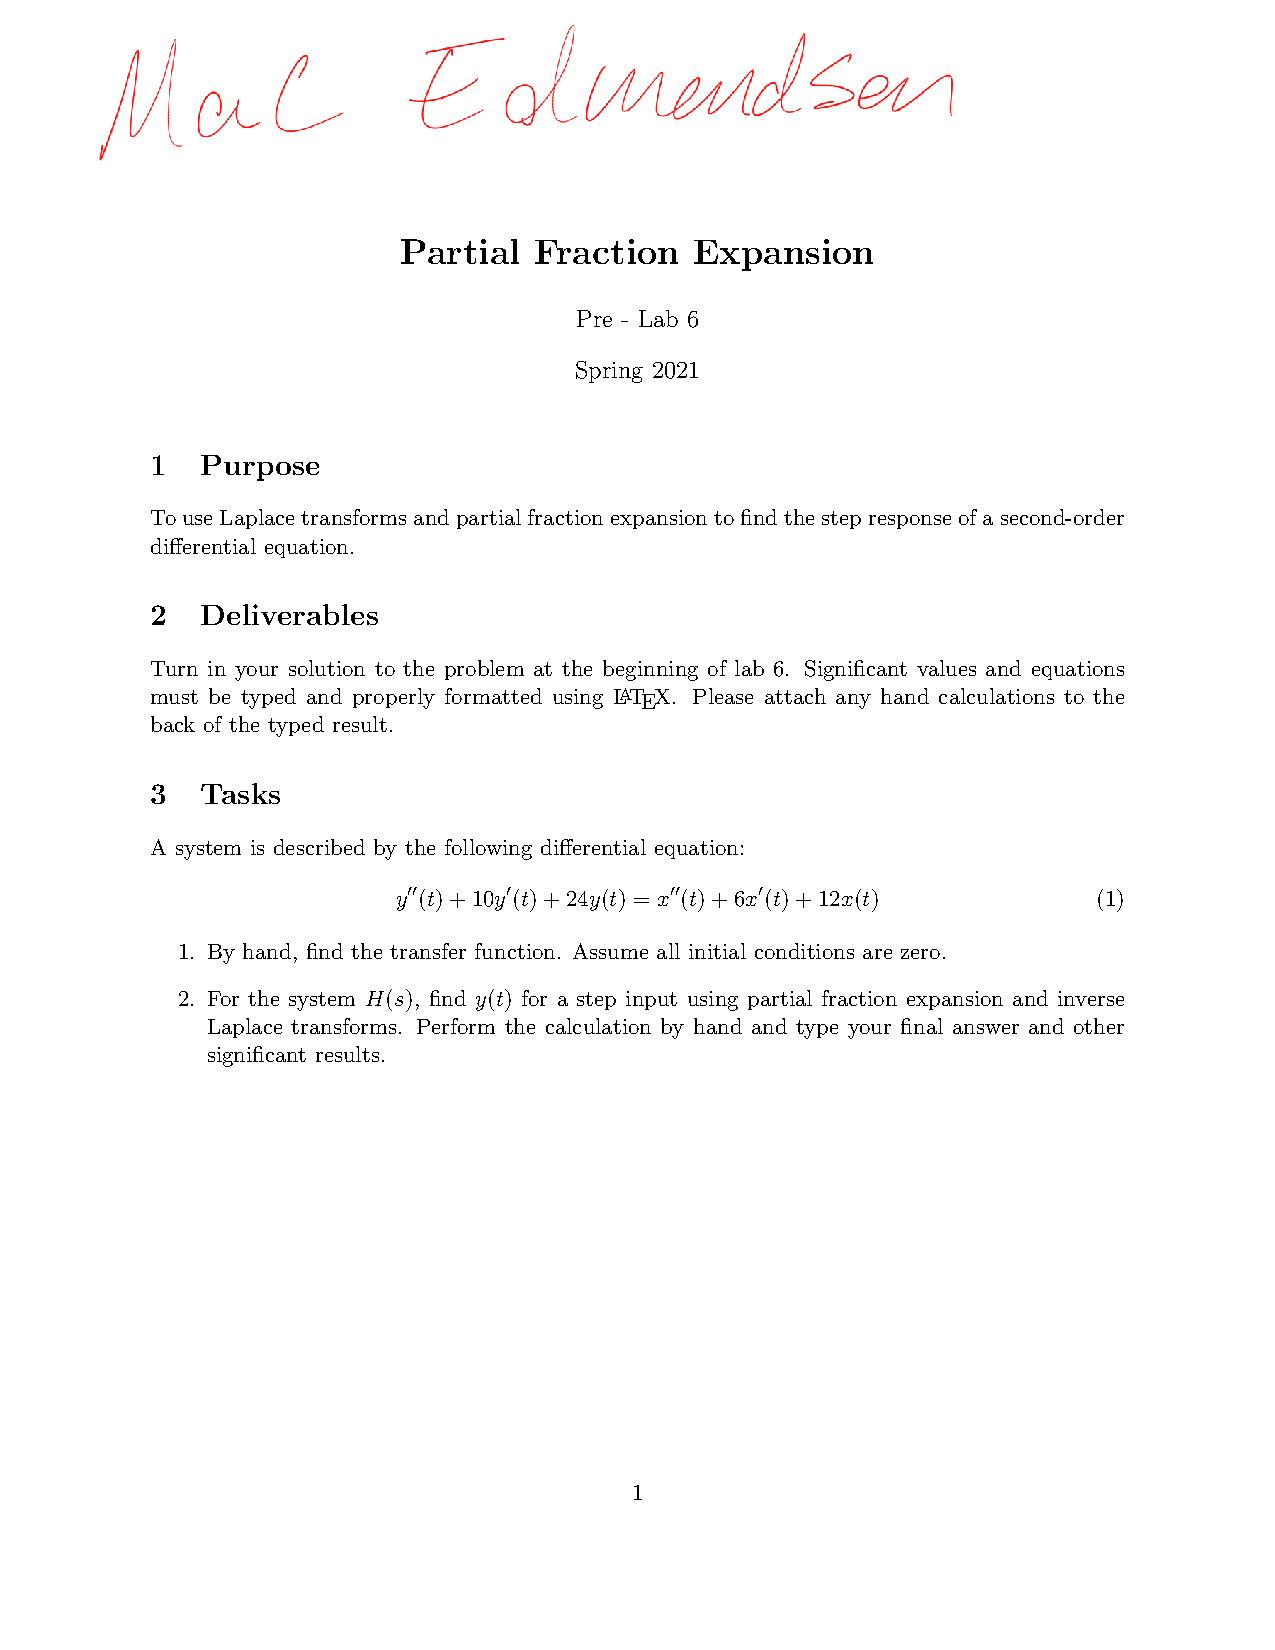
\includepdf[pages=-, offset=1in -1in]{./attachments/lab6_pre.pdf}
% \includepdf[pages=3, offset=1in -1in]{./attachments/lab5.pdf}

% \begin{thebibliography}{111} 
% \thispagestyle{customplain}

% \end{thebibliography}
\end{document}
%This template was created by Roza Aceska.